\documentclass[11pt]{article}
\usepackage[a4paper,margin=22mm,headheight=16pt]{geometry}
\usepackage{fontspec,xeCJK,xcolor,graphicx,enumitem,fancyhdr,titlesec}
\usepackage{hyperref}
\IfFontExistsTF{Times New Roman}{\setmainfont{Times New Roman}}{\setmainfont{TeX Gyre Termes}}
\IfFontExistsTF{FangSong}{\setCJKmainfont[AutoFakeBold=2]{FangSong}}{\IfFontExistsTF{仿宋}{\setCJKmainfont[AutoFakeBold=2]{仿宋}}{\IfFontExistsTF{FandolFang-Regular.otf}{\setCJKmainfont[AutoFakeBold=2]{FandolFang-Regular.otf}}{\setCJKmainfont{FandolSong-Regular.otf}}}}
\definecolor{ink}{HTML}{173747}\definecolor{accent}{HTML}{227E82}
\hypersetup{colorlinks=true,urlcolor=accent,linkcolor=accent}
\linespread{1.22}\setlength{\parindent}{0pt}\setlength{\parskip}{6pt}
\setlist[itemize]{leftmargin=1.4em,itemsep=3pt}
\titleformat{\section}{\large\bfseries\color{ink}}{}{0pt}{}
\titlespacing*{\section}{0pt}{14pt}{7pt}
\pagestyle{fancy}\fancyhf{}\lhead{\small OMNI LEARNING / 学习手册}\rhead{\small Source-grounded learning}\cfoot{\small\thepage}
\emergencystretch=2em\widowpenalty=10000\clubpenalty=10000
\newcommand{\Needspace}[1]{\par\begingroup\dimen0=#1\relax\vskip0pt plus\dimen0\penalty-100\vskip0pt plus-\dimen0\vskip\dimen0\penalty9999\vskip-\dimen0\vskip0pt\endgroup}
\begin{document}


{\LARGE\bfseries\color{ink} 辨认亮点：恒星、行星与手机星图}\par

2026-10-09 | Day01/3 | 阅读 11 分钟 + 练习 4 分钟\par\vspace{6pt}

\Needspace{5\baselineskip}\section*{今天学完，你能做什么}

旅行时抬头看到一个很亮的点，你可能会问：“它是恒星，还是行星？”今天练习把这个问题拆成两步：先记下观察线索，再用设置正确的星图核对。

用时约15分钟：起点自问1分钟，阅读与看图8分钟，必做练习4分钟，自检与回顾2分钟。用时为估算，选读和夜间观察另计。只用肉眼和已有手机星图，不购买器材。[S6]

先花1分钟想一想：你现在会不会把“很亮”或“不闪烁”直接当作行星的证明？先记下想法，暂不急着改答案。

\Needspace{5\baselineskip}\section*{概念一｜同样是亮点，光从哪里来}

恒星是自身发光的天体，太阳就是恒星。像太阳这样处在主序阶段的恒星，核心的核聚变释放能量；今天只记住“自身发光”，不需要学习反应公式。[S1]

本课讨论的太阳系行星围绕太阳公转，金星、木星和地球都是行星。月球围绕地球，是天然卫星；不能把所有反光的天体都叫作行星。[S6]

我们肉眼观看太阳系行星时，看到的主要是它们反射的太阳光。例如，金星可以反射很大一部分照到它的阳光，因此它很亮也不意味着它是恒星。这一比较说的是肉眼可见光，不是说行星没有任何形式的辐射。[S2]

看下图左栏：观测者看到的都是点状亮光，并拿手机核对。请找出“裸眼观察”和“星图确认”两个动作。仅凭这幅示意图，你无法给某个点取名字；它没有真实坐标，也不代表某一晚的天空。中、右栏仅保留课程路线，本课不学习它们。

\begin{center}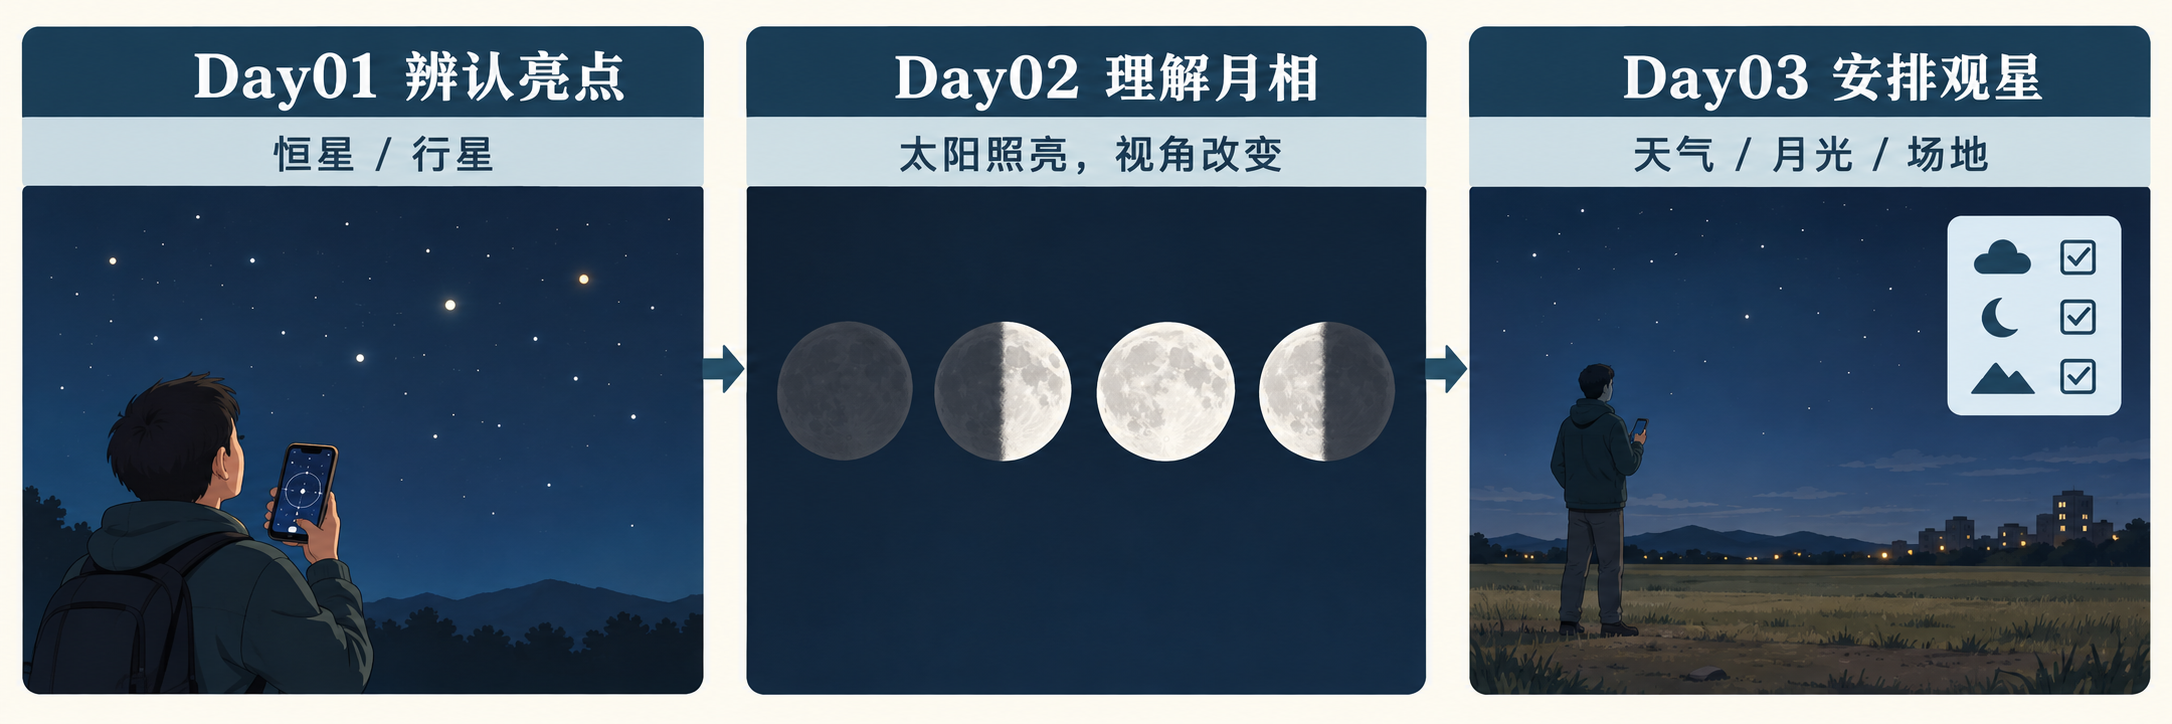
\includegraphics[width=\linewidth,height=0.26\textheight,keepaspectratio]{../assets/figure-7338e8d8739e.png}\par

{\small 图1｜本课只看左栏：为什么观察者还要看手机？因为点状外观不足以确认身份，需核对星图设置与位置。[S5][S6]}\par

{\footnotesize 复用2026-10-09由image\_gen实际生成的教学插图，非照片、非官方星图或原始证据。原始提示词和本次复核见research/Day01/image-record.json。}\end{center}

\Needspace{5\baselineskip}\section*{概念二｜闪烁是线索，不能单独定身份}

星光穿过不断变化的大气，受到扰动，肉眼会看到闪烁。恒星非常遥远，呈近似点状；行星虽然肉眼也像点，其光来自一个小的视圆面，大气扰动的影响更容易互相平均，因此行星通常显得较稳定。[S3]

这里的“视圆面”是它在天空中占据的一小块角度，并不表示肉眼一定能看到圆盘。不要把插图中亮点的大小当成真实天体的大小。[S3]

所以，“很亮、闪得少”可以帮助你挑选待核对目标，不能直接推出“这就是金星”。行星亮度会变化，也会相对背景恒星逐渐改变位置；辨认需要多项信息一起对应。[S4]

\Needspace{5\baselineskip}\section*{概念三｜星图要与眼前天空对应}

手机星图可以帮助辨认，但先检查三项：地点是不是观察地点；日期与时间是不是观察时刻；地图方向是不是你面对的方向。应用自动定位或自动取时后，也要核对显示值。[S5][S6]

方向符号N、E、S、W分别对应北、东、南、西。再看目标大概有多高：地平线附近约为0度，头顶约为90度。先理解“靠近地平线、半空、头顶”的区别即可，不必测量精确角度。[S5]

以后真正在旅行中辨认时，可以用这样的顺序：记下方向和大致高度，检查星图设置，读出该位置的标签，再核对周围的亮点是否对应。星图给出候选身份；没有可靠对应时，记录“暂未确认”。本课只检查功能入口，不预测具体日期地点的可见天象。

\Needspace{5\baselineskip}\section*{示例｜从“像行星”到“有依据地确认”}

以下是假设情境，不是现场观测：你看到一个较亮、闪烁较少的点；星图在对应位置标出“金星”。

第一步，只记“可能是行星”，因为外观线索还不够。第二步，核对星图地点、日期时间与朝向。第三步，对照大致高度和附近亮点。都对应时，可以把它记为“经星图核对的金星”；若发现时间停在另一天，就先修正设置，不能沿用刚才的判断。[S5][S6]

这是一种用于入门的核对方法，不保证仅凭一次手机指向就绝对准确。你没有看清或无法对应，也是一条有用记录。

\Needspace{5\baselineskip}\section*{必做练习｜4分钟，先做再看答案}

第1分钟：判断两个情境，各写一句理由。
A．一个点很亮且不明显闪烁。可以直接断定它是行星吗？
B．星图标成“木星”，但显示的观察时间不对。可以据此确认你眼前那个点就是木星吗？

第2至3分钟：打开已有手机星图，找到地点、日期时间、方向显示三个入口，写下在哪里查看。只看入口，不必选择某个天体或作天象预测。两分钟内没找到的项目标“未找到”，后续反馈，不继续占用今天的预算。

第4分钟：用下面三行写自己的辨认卡。
恒星和行星的区别是：\_\_\_\_\_\_\_\_。
闪烁可以提供\_\_\_\_\_\_\_\_，但不能证明\_\_\_\_\_\_\_\_。
核对身份前，我要检查\_\_\_\_\_\_\_\_、\_\_\_\_\_\_\_\_、\_\_\_\_\_\_\_\_。

练习可以坐在室内完成；不要求今晚外出，也不要求实际看到某颗行星。

\Needspace{5\baselineskip}\section*{自检答案与回顾｜2分钟}

A．不能。亮度和闪烁只是观察线索，需要星图和方向等信息一起核对。[S3][S4]
B．不能。先把时间与观察时刻对应，再重新核对位置；错误设置下的标签不能证明身份。[S5]

辨认卡参考：恒星自身发光；本课讨论的太阳系行星在肉眼可见光下主要反射阳光。闪烁提供辨认线索，不能单独证明天体身份。先核对地点、日期时间和方向。[S1][S2][S5][S6]

合格自检：你能说出发光方式的区别，能解释“不闪烁不等于已确认”，并能列出至少两项星图设置。手机入口没找到时，概念可以先学会，操作卡点另记；不要把未找到写成已完成。

今天只带走一句话：先观察，再核对，没把握就保留“未确认”。下一课将从“月亮也反射阳光”这个连接点理解月相；本轮到这里结束。

\Needspace{6\baselineskip}\section*{扩展学习 / Further reading}\small 以下为选读，不计入每日必做时间。\begin{enumerate}[leftmargin=1.6em]

\item [S1] \href{https://science.nasa.gov/universe/stars/}{恒星为什么会发光（Stars）} — 选读开头与Life第一段：认识太阳也是恒星，以及主序恒星的能量来源；不必阅读全部演化过程。\par NASA Science | 发布：未标注 | 核验：2026-10-09

\item [S2] \href{https://science.nasa.gov/moon/moonlight/}{反射光也能很亮（Moonlight）} — 只读Albedo中月球、地球与金星的比较：金星反射阳光，说明“很亮”并不证明是恒星。\par NASA Science / Caela Barry；科学顾问John Keller、Bill Farrell | 发布：未标注 | 核验：2026-10-09

\item [S3] \href{https://imagine.gsfc.nasa.gov/ask\_astro/night\_sky.html}{恒星闪烁、行星较稳定的原因} — 在页面查找“Why do the stars appear to twinkle”：读Question ID 981217a的回答，理解大气扰动和行星光线的平均效应。问题提交日期不当作回答发布日期。\par NASA GSFC / Koji Mukai、Maggie Masetti | 发布：未标注 | 核验：2026-10-09

\item [S4] \href{https://science.nasa.gov/skywatching/}{夜空中的行星与恒星} — 只读What to Look for in the Sky的Planets和Stars：对比亮度、闪烁与背景位置，跳过当月天象栏目。\par NASA Science | 发布：未标注 | 核验：2026-10-09

\item [S5] \href{https://www.jpl.nasa.gov/edu/resources/project/find-planets-in-the-sky/}{设置星图并寻找行星} — 选读步骤3、5、6：检查地点、日期时间、方向和高度。只学核对流程，不必执行指定夜晚的观测或后续预测步骤。\par NASA JPL Education | 发布：未标注 | 核验：2026-10-09

\item [S6] \href{https://science.nasa.gov/skywatching/faq/}{肉眼观星和手机星图常见问题} — 读What tools do I need和Can I see...：理解不需要购置器材，以及星图必须对应观察地点和时间。\par NASA Science | 发布：未标注 | 核验：2026-10-09

\end{enumerate}

\end{document}